\chapter{NP-Completeness}

\begin{descr}
  Definition and analyisis of different complexity classes
\end{descr}

\section{Motivation/Examples}
\begin{tabular}{p{5cm}|p{5cm}}
  Solvable in Polinomial Time & NP complete \\
  \hline
  \deftxt{Euler Path} "a path with all edges" & \deftxt{Hamiltonian Path} "node ocurs exactly once" \\
   Shortest path from X to Y $\Rightarrow$ \deftxt{Dijkstra's}algorithm & longest simple Path between X and Y \\
  \hline
  2-CNF (conjuntive normal form) e.g. $(x_{1} \lor \lnot x_{2}) \land (\lnot x_{1} \lor x_{3})$ Can we find an assignment, that the formula becomes true in poly. time? & 3-CNF \\
  \hline
  Two processor scheduling & 3 or more processor schedulung $\Rightarrow$ NP-complete or unknown \\
  \hline
  Football game until 1955 loss 0 points, draw 1 point, win 3 points. The season has already started, is my team still able to win the championchip? & loss 0 points, draw 1 point, win 3 points \\
\end{tabular}

\section{Introduction}
\begin{definition}
  P is the class of problems that can be solved in polinomial time.\\

  NP is the class of porblems, where given a solution one may check in polinomial time, that it is indeed one.
\end{definition}

\begin{example}
Example:
\begin{enumerate}
  \item Given a connected undirected-finite graph. Is there a circle such taht every node appears exatly once on the circle.
        Given such a circle $< v_{1},...v_{n}>$ it can easily checked that it has the property. $\Rightarrow$ Hamiltonian Cycle $\in$ 
        NP.
  \item 3-CNF; given values for the variables, we can check that the formula becomes true, with this values in polynomial time.
\end{enumerate}

\textbf{Clarity:} $P \subseteq NP$ open problem; $P = NP ??$

Overview: \\
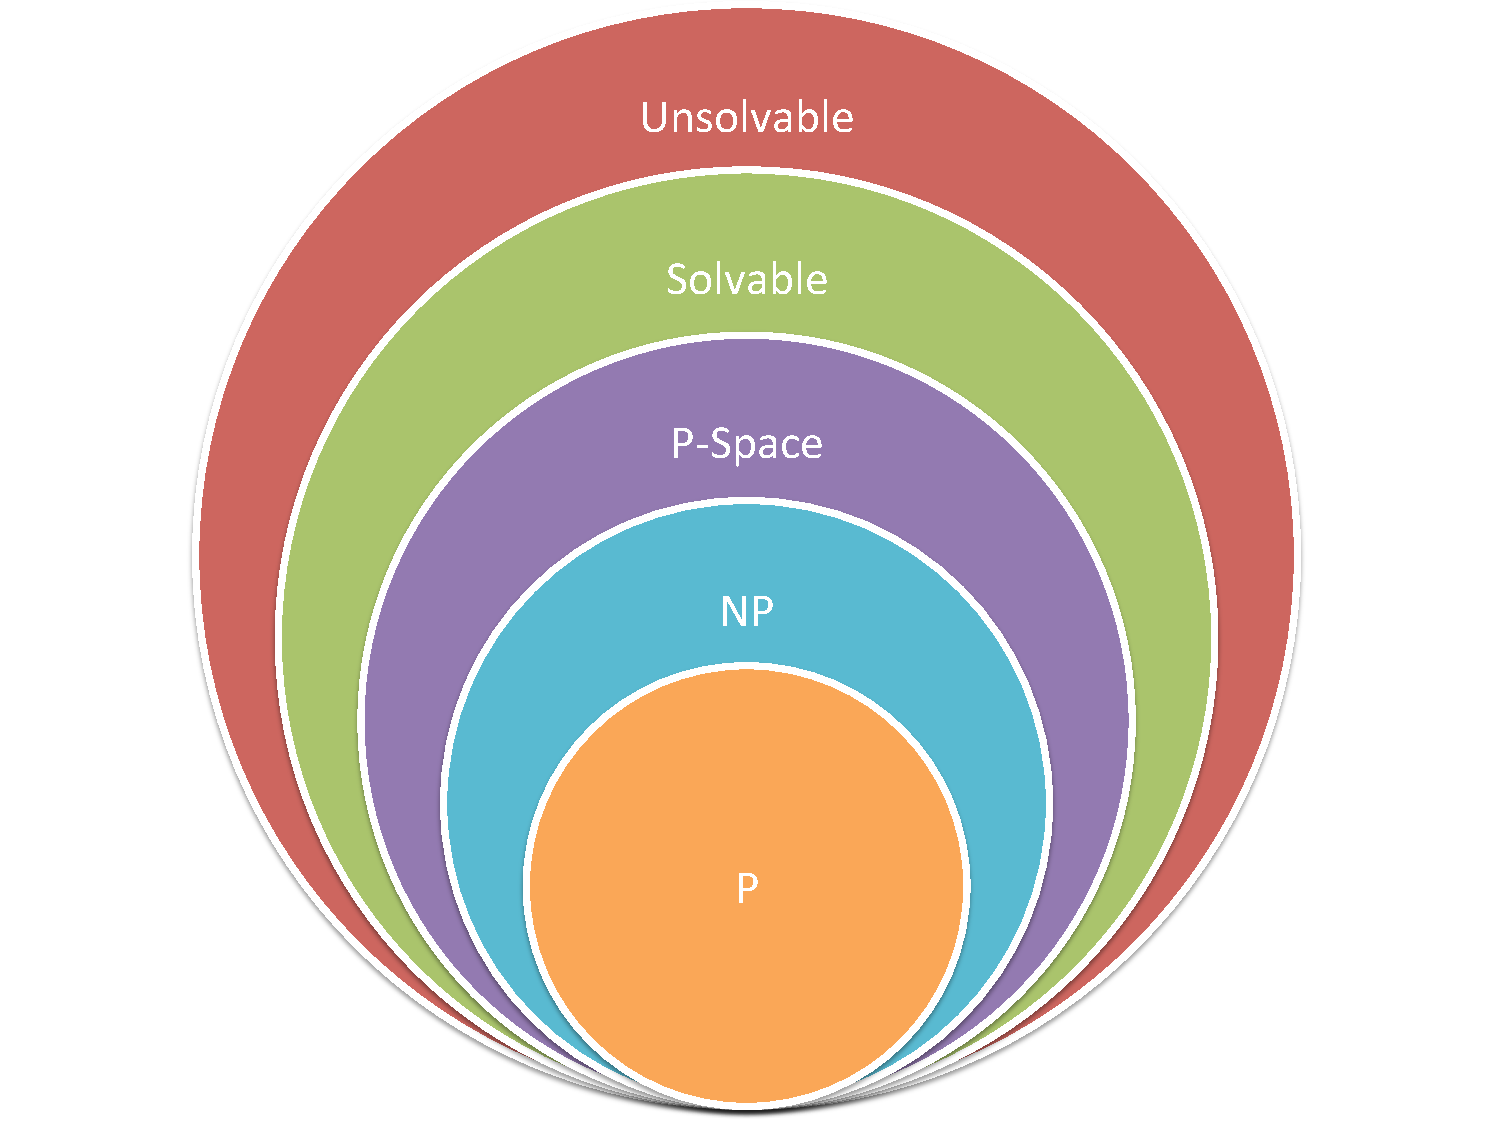
\includegraphics[scale=0.3]{diagrams/comp_classes}
\end{example}

\section{Problem Types/Issues}

\begin{tabular}{p{5cm}|p{5cm}}
  \textbf{Decision Problems} & \textbf{Optimization Problems} \\
  \hline
  Yes or no answer, is there a path from X to Y? & Find the shortest path from X to Y?
\end{tabular}

\begin{definition}
  Complexity Theory deals with \deftxt{decision problems}. Optimization problems are tried to transform into decision problems.
\end{definition}

\begin{example}
  Choose an integer k, treat the decision problem: "Is there a path from X to Y no longer than k?"
\end{example}  

To show that an optimization problem is hard to solve it is sufficient to consider the related decision problem. If the latter is hard to solve, so is the first. \\

\textbf{Reductions} \\
Reductions are used to show that problem are hard to solve. A reduction reduces a decision problem to another one.\\
$A \Rightarrow B$ (reduction)

Properties of the reduction should be: "it can be done in polynomial time". \\
If $A$ and $B$ the transformation of $A B$ is an instance of $B$ then $A$ should have the answer yes if and only if $\beta$ has the answer yes.\\
Call this a \deftxt{polynomial reduction}.\\
If $A \rightarrow B$ and $B$ can be solved in poly. time, then instances of $A$ can be solved in poly. time. \\
If $A \rightarrow B$ and $A$ is hard to solve, then we may conclude that  $B$ is hard to solve. \\

